% !TEX spellcheck = en_US
% !TeX program = pdflatex
% !TeX TXS-program:bibliography = txs:///bibtex
% !BIB program = bibtex

%% LMU-MI-HS-Template
%% This template is an adaptation of the IEEE InfoVis/Vis format
%% http://www.cs.sfu.ca/~vis/Tasks/camera_tvcg.html
%% Last update: Bastian Pfleging, 05.2016

\documentclass[journal]{vgtc}                % final (journal style)
\usepackage[english]{babel}
\usepackage{mathptmx}
\usepackage{caption}
\usepackage{mdframed}
\usepackage{graphicx}
\usepackage{times}
\usepackage[hyphens]{url}
\usepackage{float}
\usepackage{dcolumn}
\usepackage[backend=bibtex, style=numeric, isbn=true, doi=true, maxnames=99]{biblatex}
% WaterMarker
\usepackage{draftwatermark}
\SetWatermarkText{second draft}
\SetWatermarkScale{1}

\addbibresource{literature.bib}

\DeclareGraphicsExtensions{.pdf,.jpg,.pdf,.mps,.png}
\graphicspath{{img/}} 


\normalfont


%% Paper title.

\title{A Literatural Overview on Explanations in Personalization and Possible Criterion for Designing a Short Explanation}

%% Put your name here
\author{Yifei Zhan}
\authorfooter{
%% change name, course (Media Informatics/Informatics/etc) and email for the footer
\item
  Yifei Zhan is studying Media Informatics at the University of Munich, Germany, E-mail: yifei.zhan@campus.lmu.de
\item
    This research paper was written for the Media Informatics Advanced Seminar ' Hauptseminar Medieninformatik', 2017
}


%% Abstract section.
\abstract{
This paper provides a literatural overview of explanations in personalization and recommender systems.
It then introduced two standards/criterion on how to design and evaluate explanations in recommender systems.
Which type of explanations the system should offer to users depends on the goal of the system.
And in some scenarios, like in a driving context, pages of explanations might not be suitable. In this case,
short explanations is preferred. In order to explore possible criterion of short explanations, two studies were
introduced and what we have found is that \textbf{efficiency}, \textbf{persuasiveness} and \textbf{why} question-type-based
explanations might be suitable for short explanations. However, some more studies need to be done in order to
check the validity of other criterion in short explanations.
} % end of abstract

%% Keywords that describe your work.
\keywords{Explanation, Recommender system, Personalisation}

%%%%%%%%%%%%%%%%%%%%%%%%%%%%%%%%%%%%%%%%%%%%%%%%%%%%%%%%%%%%%%%%
%%%%%%%%%%%%%%%%%%%%%% START OF THE PAPER %%%%%%%%%%%%%%%%%%%%%%
%%%%%%%%%%%%%%%%%%%%%%%%%%%%%%%%%%%%%%%%%%%%%%%%%%%%%%%%%%%%%%%%%

\begin{document}
\maketitle
\section{Introduction}

  \indent Personalization is no more a novelty. The first emergence of this phenomenon dated back to antiquity
  when experienced merchants provided different customers with different products or services \cite{adomavicius2008personalization}. However, the real interest of personalization did not arise until the late 1990s with the advancement of the Web technologies \cite{don2011managing}.
  From then on, more studies have been done in this field, and people try to explore the essence of personalization.

  \indent In the world of personalization, one thing we might often hear about is recommender systems (RS), which intelligently give users personalized suggestions. The recommendations can vary from algorithm to algorithm. The most common forms are the content-based recommendation, and the collaborative filtering recommendation. The first one, content-based recommendation, observes utility of previous items and then use this attribute to predict the utility of other items \cite{balabanovic1997fab}. An example can be ``User A has bought a novel. And based on this bought history, a magazine is more likely to be recommended to him than a pair of shoes, because novels and magazines are more in common than novels and shoes ''. The second type, collaborative filtering, observes utility for user-item pairs which is then used to predict utility for unobserved user-item pairs \cite{balabanovic1997fab}. One example can be ``User A(1,2) has bought items 1 and 2, user B(1,2,3) has purchased items 1,2 and 3 and user C(2,4) has bought items 2 and 4. As a recommendation for user A, item 3 is more likely to be suggested to user A than item 4, since user A and user B are more similar than user A and user C''.

  \indent A good recommendation algorithm is no doubt indispensable for a recommender system, and the way of explaining its complex algorithm to users
  plays also an important role. With the development of the Internet, the privacy issue becomes more and more important. The newly EU regulation even requires explanations for complex algorithms \cite{goodman2016european}. People are willing to know which information is ``consumed'' by the system and they may lose their trust in one system if it behaves differently as they expected. 
  In this case, a proper explanation of a recommender system can help to inspire users' trust and loyalty, increase satisfaction, make it quicker and easier for users to find what they want \cite{tintarev2007survey}. In order to answer the question, "What makes a good explanation," we check through different studies and try to summarize a set criteria in this paper. Besides, we particularly focus on brief explanations.

  \indent The rest of the paper is divided into four parts. The first section provides an overview of different studies on explanations in recommender systems. The second part focuses on two frameworks, which are often used by other researchers to evaluate and design explanations of recommender systems. The third section extracts some principles from the two frameworks, which can be used to design ``brief explanations'' in an automotive scenario. And in the last part, we summarize our contribution and propose several questions for future studies.

\section{Literature Review}

    \indent In this section, we try to give readers an overview of state of the art. We introduce in this part some relevant studies which focus on the recommendation and its explanations.

    \indent User experience research is increasingly attracting researchers’ attention. Some researchers, like Li Chen \cite{pu2011user}, and Bart P.Knijnenburg \cite{knijnenburg2012explaining}, put emphasis on recommender system and try to figure out what constitutes an effective and satisfying recommender system. Other researchers focus on its explanations. They have proved that a good explanation can boost users' trust towards the system and help them in decision making process \cite{tintarev2007survey} \cite{van2004designing} \cite{pu2007trust}.
    
    \indent One possible way to evaluate explanations of a recommender system is to look at the soundness and completeness \cite{kulesza2013too}. The soundness means the extent to which an explanation describes all of the underlying systems. Meanwhile, the completeness means how truthful each element in an explanation is, in the perspective of a user, in the underlying system. The author has found out that LSHC(which means low soundness and high completeness) provides participants with the best-perceived cost/benefit ratio of attending to the explanations. 

    \indent Another possible method to evaluate the explanations is to categorize explanations in different types of questions. In Lim's work, Toolkit Support Intelligibility in Context-Aware Applications \cite{lim2010toolkit}, they divided the explanation of a context-aware system into eight questions, which are Why, Why Not, How To, What, What If, Inputs, Outputs, and Certainty. In the findings, they emphasized on streamlining explanations while maintaining access to the rich explanation capabilities, which makes explanations usable and quickly consumable.    
    
    \indent Finally, a significant breakthrough is made by Nava Tintarev and Judith Masthoff. They have proposed what they called ``seven possible advantages of an explanation facility \cite{tintarev2007survey}.'' These seven advantages are often taken as a standard criteria in evaluating and designing explanations for a recommender system.

\section{Explanatory Criterion and two Types of Explanation}
\subsection{Seven Explanatory Criterion}
    \indent The explanatory criterion\cite{tintarev2007survey} (see table \ref{table:1}), originally proposed by Nava Tintarev and Judith Masthoff, 
    are mostly used when considering to design the explanation of a recommender system. 

    \begin{table}[ht] 
        % ht used to attach the table to the position approximately where they are wrote here
        \centering
        \begin{tabular}{ | m{8em} | m{4cm} |} 
        \hline
        %  \bfseries used to bold the header
         \bfseries Aim & \bfseries Definition\\ [0.5ex] 
        \hline\hline
        Transparency & Explain how the system works\\ 
        \hline
        Scrutability & Allow users to tell the system it is wrong\\ 
        \hline
        Trust & Increase \text{users\textquotesingle} confidence in the system\\ 
        \hline
        Effectiveness & Help users make good decisions\\ 
        \hline
        Persuasiveness & Convince users to try\\ 
        \hline
        Efficiency & Help users make decisions faster\\ 
        \hline
        Satisfaction & Increase the ease of use or enjoyment\\ 
        \hline
        \end{tabular}
        \caption{Explanatory criteria and their definitions}
        \label{table:1}
    \end{table}
    \indent Although they have different names in different researches. For example, 
    Mohammed Z.Taie call them explanation attributes\cite{al2013explanations},
    which represent the benefits explanations provide to recommender systems and Fatih Gedikli call them quality factors, 
    which he used to evaluate different explanation types in his study\cite{gedikli2014should}.
    They have the same purpose, that is, to make the system more understandable by users.
    These criterion are listed here as follows:
    
    \begin{enumerate}
        \item \textbf{Transparency:} TODO:// write the intro
        \item \textbf{Scrutability:} TODO:// write the intro
        \item \textbf{Trust:} TODO:// write the intro
        \item \textbf{Effectiveness:} TODO:// write the intro
        \item \textbf{Persuasiveness:} TODO:// write the intro
        \item \textbf{Efficiency:} TODO:// write the intro
        \item \textbf{Satisfaction:} TODO:// write the intro
    \end{enumerate}

\subsection{Type 1 -``Detailed Explanation''}
    TODO: The definition of Detailed Explanation?
    Most of the recommender systems on desktop scenario adapted the ``Detailed Explanation''.
    They covered almost all of the seven explanatory criterion that mentioned above......TODO: complete the intro part
\subsection{Examples for ``Detailed Explanation''}
    An example of explanation in amazon.com.
    TODO: (Write Analysis based on seven explanatory criterion) 
    \begin{figure}[H]
        \centering
        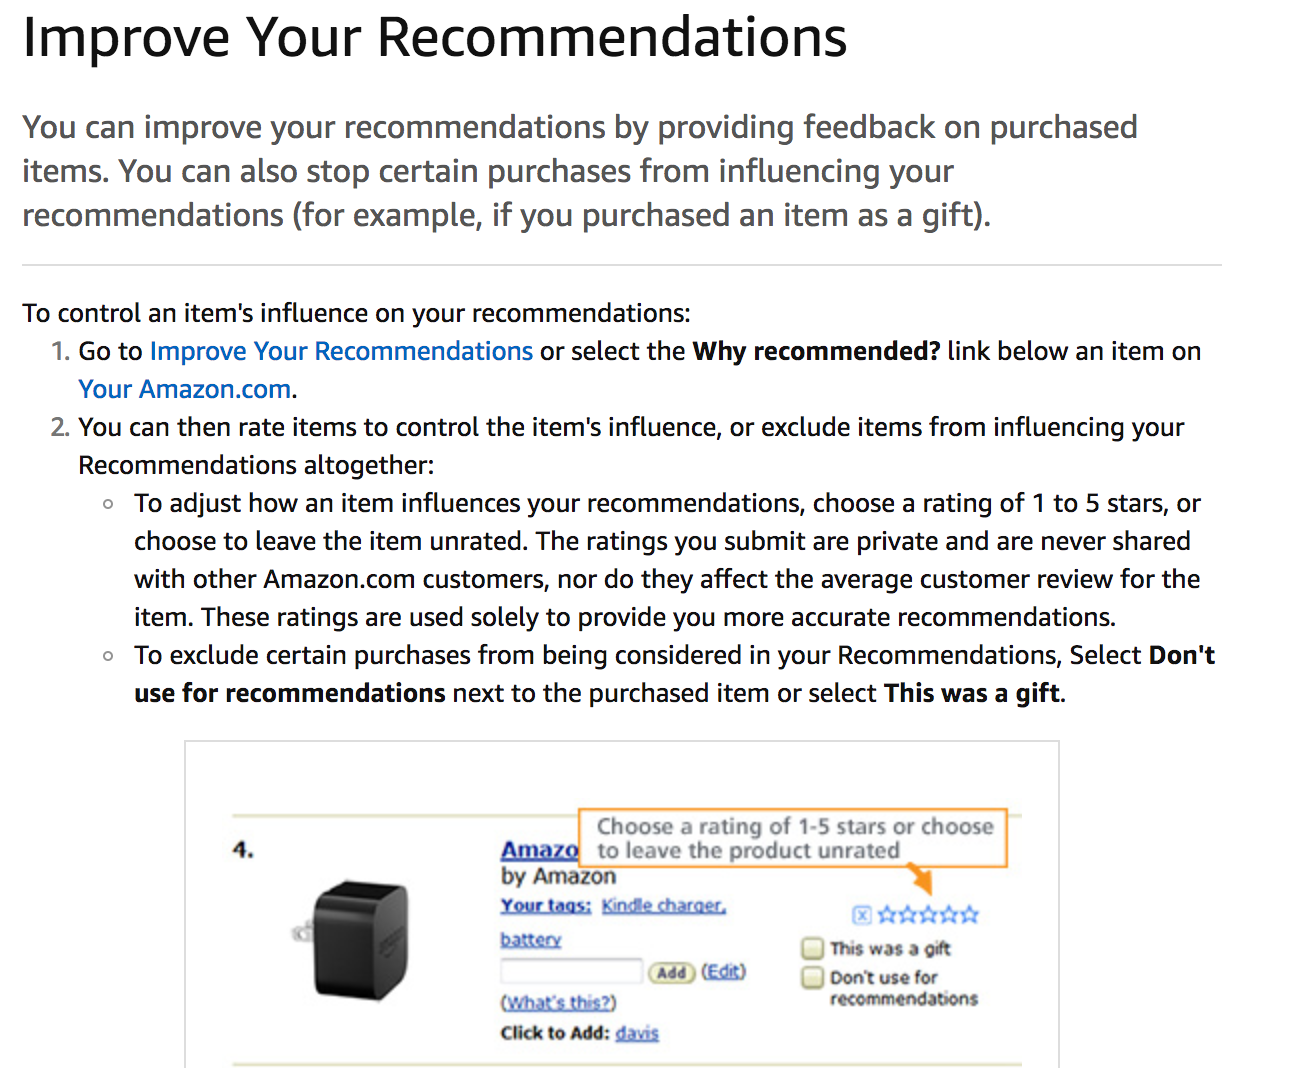
\includegraphics[width=0.5\textwidth]{figures/amazon1}
        \caption{Amazon}
        \label{fig:amazon1}
    \end{figure}
    An example of explanation of Google Ads.
    TODO:  (Write Analysis based on seven explanatory criterion) 
    \begin{figure}[H]
        \centering
        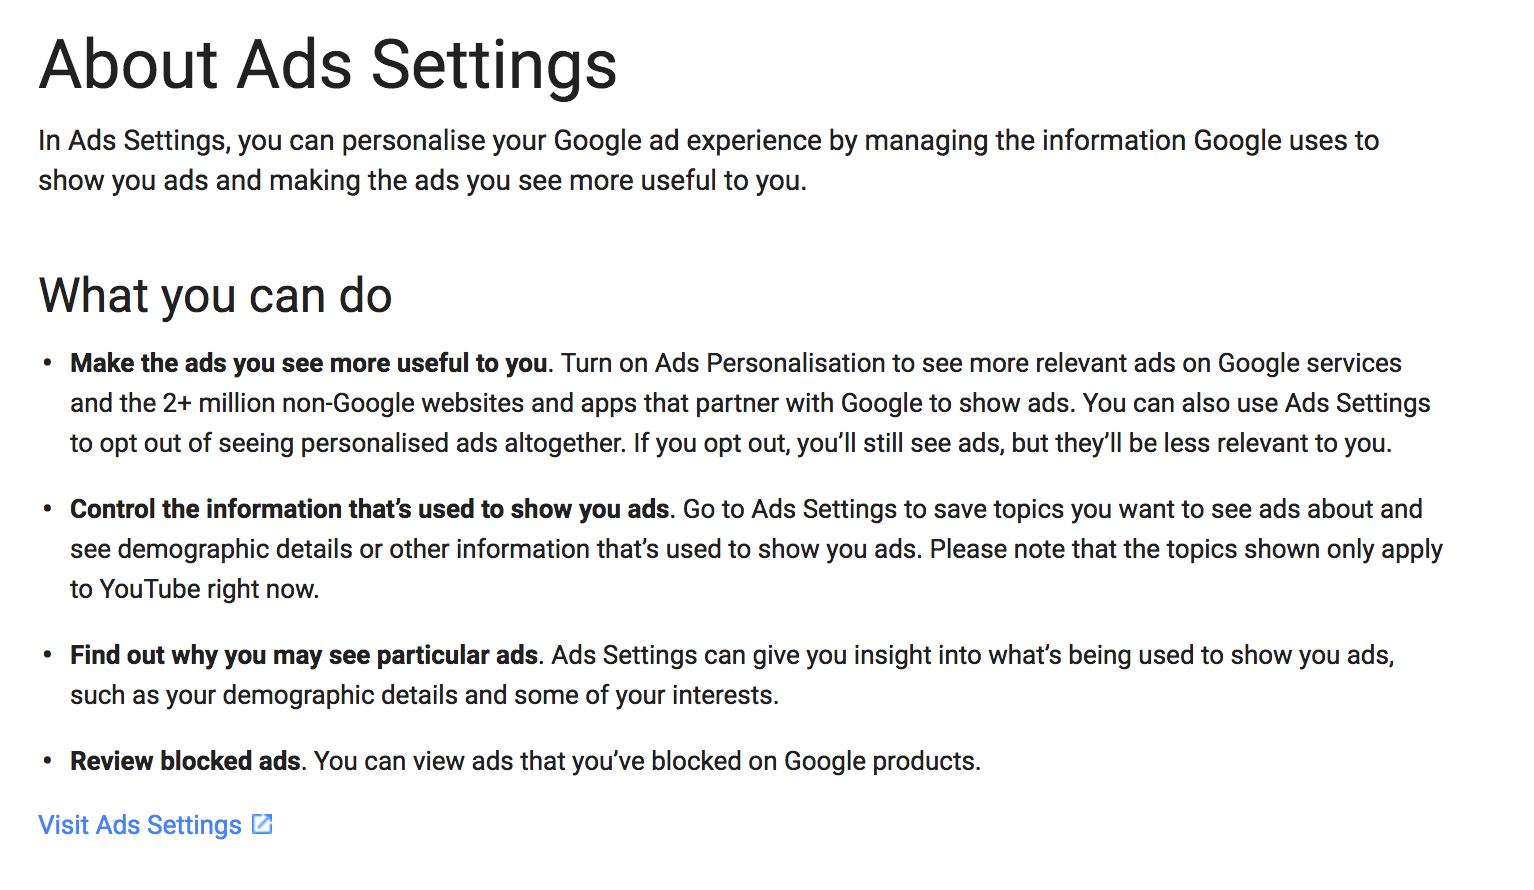
\includegraphics[width=0.5\textwidth]{figures/google1}
        \caption{Google}
        \label{fig:google1}
    \end{figure}
\subsection{Type 2 -``Brief Explanation''}
    However, in some scenario, a brief explanation is more suitable, for example, driving in a car
    (why: users have limited attention resource)
    We can not take all seven explanatory criterion into consideration.
    How to extract a kind of standards.
\subsection{Examples for ``Brief Explanation''}
    Example1: Explanations in Proactive Recommender Systems in Automotive Scenarios \cite{bader122011explanations}
    \textbf{Extract two criterion out of seven explanatory criterion: Persuasiveness and Efficiency.}

    Example2: Why did my car just do that? Explaining semi-autonomous driving actions to improve driver understanding, trust, and performance\cite{koo2015did}
    \textbf{Extract two types (what and how)based on question types from Intelligent Toolkit} \cite{Brian2010toolkit, lim2011design}
\subsection{Comparison between ``Detailed Explanation'' and ``Brief Explanation''}

\section{Discussion, Future Work and Conclusion}

    \indent With the development of the automobile and mobile industry, more and more recommender systems need to work in a context-aware environment and compared with the desktop environment, users can not fully concentrate on the device because their environment requires more attention at the same time. In such cases, an efficient and brief explanation which informs the system's behaviors is especially important.
    
    \indent However, unlike typical explanations in a recommender system (explanations for desktop recommender systems), which has already some ``standard'' methods to design them. There is no ``standard'' approach to design and evaluate brief explanations. 

    \indent In the first study, mentioned in section 4.1, Roland Bader extracted two criteria from the first framework - Seven Explanatory Criteria for brief explanations. He has successfully proved that these two principles (\textbf{efficiency} and \textbf{persuasiveness}) from the first framework are suitable for brief explanations. However, he did not mention other principles. Thus, it might be helpful if further studies can examine and evaluate other criteria (\textbf{transparency}, \textbf{scrutability}, \textbf{effectiveness}, \textbf{trust} and \textbf{satisfaction}). In the second study,  Martin Steinert only evaluated two types of explanations (\textbf{what} and \textbf{why}) extracted from the second framework, Question-Based-Explanation. Therefore, some further studies can focus on other question-type-based explanations (\textbf{why not}, \textbf{how to}, \textbf{what if}, \textbf{inputs}, \textbf{outputs} and \textbf{certainty}).

    \indent In conclusion, in this paper, we firstly provided a literature overview of explanations in personalization and recommender systems. Secondly, we introduced two frameworks (Seven Explanatory Criteria and Question-Type-Based Explanations) which are used to design and evaluate explanations. Moreover, we illustrated how these two frameworks are applied in Google Advertisement recommender system. Thirdly, we introduced two studies which extracted some principles (\textbf{efficiency}, \textbf{persuasiveness} and \textbf{why} question-type-based explanations) from the two frameworks mentioned above, in order to find a proper approach to design brief explanations for a assistant recommender system in a car. And finally, we summarized our contributions and proposed some possible directions for future studies.
%% Do not change the following:
%\bibliographystyle{abbrv}
\printbibliography
\end{document}
